%!TEX root = ../bachelors_thesis.tex

\section{Model Overview}
For the implementation of this algorithm there was only one model that truly stood out in the sense of object orientated programming. For all other functions it proved rather difficult to find a clear class where it belonged to and also making good use of responsibilities of those classes. As mentioned in chapter \ref{chap: Justification Logic} the main work was done using syntax trees and so it was the most obvious class to build. I decided to make a extra class for the \emph{Nodes} where all the small things like setting a child, and checking if it is a root and such would be handled. \emph{Tree} and \emph{Node} could have been merge to be one class only but I found it easier to work with the code if the more standard and trivial stuff of binary trees was separated from what was more specific for this algorithm. A lot of the \emph{atomize} part is handled by the \emph{Tree} class since it works within the formula and also changes the structure of it.

The most important class however is the \emph{ProofSearch} class. It acts as a sort of main class as the initialization of the formula and the cs-list takes place here. It is also here that the methods of the \emph{Tree} class are called from. Its responsibility is to handle all algorithmic task that can be done without using a syntax tree. So the major logic of the conquer step is implemented here.

Last there is the typical \emph{Helper} class. The methods here are usually rather short  and simple and serve the purpose of making the \emph{Tree} and \emph{ProofSearch} class appear cleaner. It may be argued that some of those methods present in \emph{Helper} should be better placed in \emph{ProofSearch} and vice a verse but then again the argument for a clean object orientated model design for an algorithm is questionable and very difficult to archive.

\begin{figure}[H]
	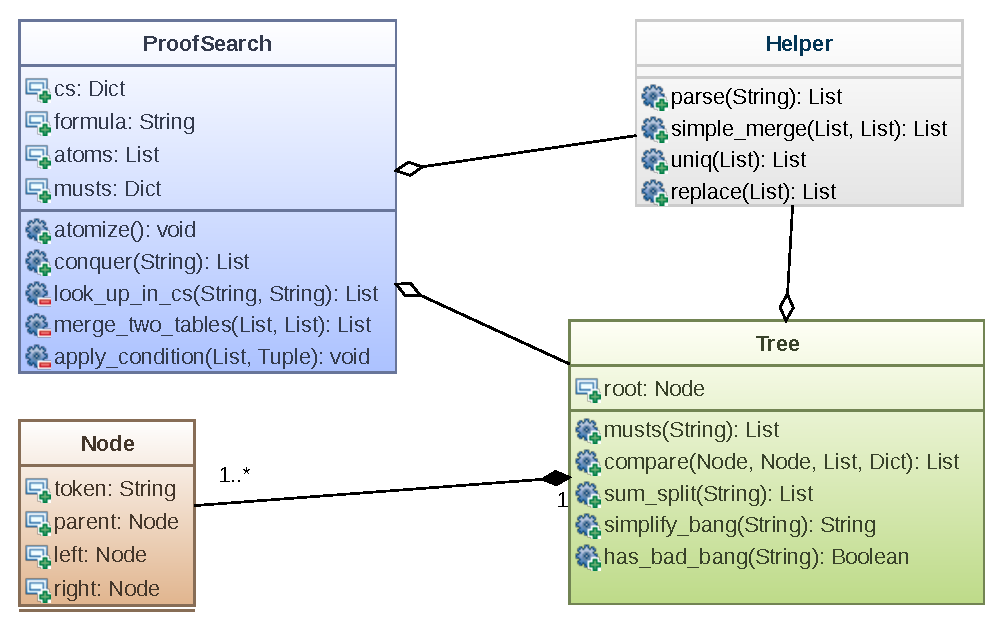
\includegraphics[width=0.9\textwidth]{/home/lyriael/BA/j-logic/thesis/Figures/uml_01.pdf}
	\caption{Simplified UML graphic of the classes used for implementing the algorithm. The list of methods and attributes is by no means complete and should simply give an idea of the construction.}
	\label{uml}
\end{figure}

\section{Operation Syntax Tree}
One of the earliest challenges was a useful representation of a formula with which I could work decently. Interestingly enough a binary tree came only later into my mind, after I tested various libraries from Python. There were libraries that seemed very useful at first as they were math-specific. Analyzing formulas that contained $*$ or $+$ were fairly easy but as $:$ and $!$ are not very common operations I could not customize the tested libraries enough to handle those as well.

So it happened while I was searching yet for another library that I tumbled over the possibility to use binary trees to represent the syntax of a mathematical formula. Remembering a lot of what I learned in the lecture about Datastructure and Algorithms I realized that this is the best choice for me. A binary tree gives me not only a way to represent a formula in a way that interprets the order of operations but with the knowledge about trees it became suddenly very easy to also manipulate such a formula for example by deleting or swapping subtrees and still keep a valid operation. 

I decided to implement my own tree for that purpose. It might be argued that a lot of work could be saved if I used available syntax trees but for one thing I relished the idea of implementing a tree structure that I would use myself and thus finally use what I have learned in lecture ages ago and second I would have to make custom changes to a finished solution anyway and those changes are probably more work than the implementation of a binary tree which is rather simple.

I tried to keep the tree as simple as possible, giving the nodes only a value and not a unique key. The greatest challenge given by implementing a syntax tree was to handle the unary operator $!$. As braces serve to determine the depth of a tree and a binary operation tells you when to start climbing up again, it required so extra case handling for the $!$ operator. From the point on when the tree was working, it was not only important to the algorithm, but could also be used to check if the input was written correctly. Therefore most of the tests that test the string handling of a tree are the result of formulas used somewhere else but which needed syntax spell checking. 


\section{Important Methods}
In this section I want to show and explain some of the more complicated methods that are important and make up the heart of the algorithm.

\subsection{musts}

The method \emph{musts} expects a given proof term to be already \emph{atomized} as it only distinguishes between $!$ and $*$ operations.
The algorithm takes the formula in form of a tree apart from top to bottom, generating new, smaller terms for every operation it takes apart until the remaining proof term is only a proof constant. Since the resolve of a $*$ operation needs a new \emph{X-wild} and the resolve of a $!$ operation replaces an existing \emph{x-wild} and therefore needs a new as well, the current $i$ for a new \emph{X-wild} $X_i$ is stored and increased in \texttt{v\_count}.

\begin{figure}[H]
    \vspace{-10pt}
	\lstinputlisting[firstline=2, lastline=22]{/home/lyriael/BA/j-logic/thesis/code_tree.py}
	\vspace{-10pt}
	\caption{Excerpt from $Tree.musts$}
	\vspace{-10pt}
\end{figure}

If for example the current justification term would be $((a*(!b)):F)$, it would be taken apart to the two subformulas $(a:(X_i\rightarrow F))$ and $((!b):(X_i))$. Because of the \emph{atomization} in the steps before it is guaranteed that every $!$ is a (right) child of a  $*$ and since every $*$ creates a new $X_i$, a term here that starts with a $*$ is always on a $X_i$. Since from $!b:X_i$ follows $\exists X_j \quad s.t. \quad !b:(b:X_j)$, all $X_i$ that occurred up to now must be replaced by $(b:X_j)$. In the end we will have only proof constants remaining.

\subsection{unify}
\todoWriteMore{Write about unify}

\subsection{simplify}
\todoWriteMore{Write about simplify}

\subsection{resolve_conditions}
\todoWriteMore{Write about resolve conditions}


\section{Tests}
The tests I have written for this algorithm have been most important to the success of it. I usually 
\todoWriteMore{Write about Tests}
